\documentclass[tikz]{standalone}
\begin{document}
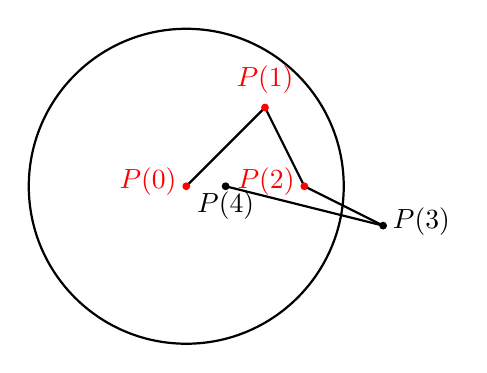
\begin{tikzpicture}[scale=0.5]
  \coordinate (p0) at (0, 0);

  \coordinate (p1) at (2, 2);
  \coordinate (p2) at (3, 0);

  \coordinate (p3) at (5, -1);
  \coordinate (p4) at (1, 0);

  \draw[thick] (p0) -- (p1);
  \draw[thick] (p1) -- (p2);
  \draw[thick] (p2) -- (p3);
  \draw[thick] (p3) -- (p4);

  \draw[thick] (p0) circle (4);

  \node[circle,fill,color=red,inner sep=1pt,label={[text=red, left]:\(P(0)\)}] at (p0) [] {}; 
  \node[circle,fill,color=red,inner sep=1pt,label={[text=red, above]:\(P(1)\)}] at (p1) [] {}; 
  \node[circle,fill,color=red,inner sep=1pt,label={[text=red, left]:\(P(2)\)}] at (p2) [] {}; 
  \node[circle,fill,color=black,inner sep=1pt,label={[text=black, right]:\(P(3)\)}] at (p3) [] {}; 
  \node[circle,fill,color=black,inner sep=1pt,label={[text=black, below]:\(P(4)\)}] at (p4) [] {}; 
\end{tikzpicture}
\end{document}
